\section{Sensitivity Methods}
%{\it Assigned to:} {\bf Elizabeth Worcester} with contributions from Chris Backhouse and Callum Wilkinson. 
\label{sec:physics-lbnosc-sens}


 %Method for calculation of sensitivity should be described. Describe previous work with Globes which might include validation of new software framework. Describe CafAna and any specifics of the DUNE fits. 

%\begin{itemize}
%\item Sensitivity Calculation Methods - Text from CDR
%\item Statistical Methods - Text from CDR 
%\item GLoBES -  EW
%\item CAFAna Methods - CB
%\item Dune fit - CW
%\end{itemize}

Sensitivities to the neutrino mass ordering, CP violation, and $\theta_{23}$ octant, as well as expected resolution for neutrino oscillation parameter measurements, are obtained by simultaneously fitting the \numutonumu, $\bar{\nu}_\mu \rightarrow \bar{\nu}_\mu$, \numutonue, and $\bar{\nu}_\mu \rightarrow \bar{\nu}_e$ far detector spectra along with selected samples from the near detector.  It is assumed that 50\% of the total exposure is in neutrino beam mode and 50\% in antineutrino beam mode.  A 50\%/50\% ratio of neutrino to antineutrino data has been shown to produce a nearly optimal \deltacp and mass ordering sensitivity, and small deviations from this (e.g., 40\%/60\%, 60\%/40\%) produce negligible changes in these sensitivities. %\todo{check this is still the case} 

In the sensitivity calculations, neutrino oscillation parameters governing long-baseline neutrino oscillation are allowed to vary. In all sensitivities presented here (unless otherwise noted) \sinstt{13} is constrained by a Gaussian prior with 1$\sigma$ width as given by the relative uncertainty shown in Table~\ref{tab:oscpar_nufit}, while \sinst{23}, $\Delta m^{2}_{32}$, and \deltacp are allowed to vary freely. The oscillation parameters $\theta_{12}$ and \dm{12} are allowed to vary constrained by the uncertainty in in Table~\ref{tab:oscpar_nufit}. The matter density of the earth is allowed to vary constrained by a 2\% uncertainty on its nominal value. Systematic uncertainty constraints from the near detector are included either by explicit inclusion of \dword{nd} samples within the fit or by applying constraints expected from the \dword{nd} data to \dword{fd}-only fits.

The experimental sensitivity is quantified using a test statistic, $\Delta\chi^2$, which is calculated by comparing the predicted spectra for alternate hypotheses.  The details of the sensitivity calculations are described in Section~\ref{sect:methods-dunefits}. 
A ``typical experiment'' is defined as one with the most probable data given a set of input parameters, i.e., in which no statistical fluctuations have been applied. In this case, the predicted spectra and the true spectra are identical; for the example of \dword{cpv}, $\chi^2_{\mdeltacp^{true}}$ is identically zero and the $\Delta\chi^2_{CP}$ value for a typical experiment is given by $\chi^2_{\mdeltacp^{test}}$. The interpretation of $\sqrt{\Delta\chi^2}$ has been discussed in \cite{Qian:2012zn,Blennow:2013oma}; it may be interpreted as approximately equivalent to significance in $\sigma$ for $\Delta\chi^2>1$. 

%Sensitivity studies are designed to test how well data will be able to distinguish between alternate hypotheses. For statistically limited data samples this process is well defined, and as long as the model gives an accurate prediction of the expected event rates, the results are easy to interpret. For systematic-limited measurements the predicted number of events is less important since they determine the sub-dominant statistical uncertainties. In this case, the specific implementation of the systematic will determine the result. Since most systematic effects induce very specific spectral changes, only ensembles of systematic uncertainties that produce effects degenerate with the parameters of interest affect the sensitivity. The freedom of the fit can be increased by creating error envelopes for systematic effects, but this technique will not allow constraints of parameters via simultaneous fits of additional samples e.g. ND samples. In the end, the results of any systematic-limited sensitivity calculation is only useful in evaluating the sensitivity for the specific case of investigated and cannot be thought of as a general result. Several techniques were used to evaluate the effects of systematic uncertainties in the studies reported in this document, and results must be interpreted carefully and with a thorough understanding of specific implementation of the systematic used.

\dword{dune} sensitivity has been studied using several different fitting frameworks. \dword{globes}~\cite{Huber:2004ka,Huber:2007ji} %facilitates the use of standardized input formats to calculate predicted spectra and defines methods that enable a test statistic to be computed given a set of inputs. The details of DUNE's GLoBES implementation have been described in \cite{Acciarri:2015uup,Alion:2016uaj,Bass:2014vta}. GLoBES
-based fits have been used extensively in the past, in particular for sensitivity studies presented in the \dword{dune} \dword{cdr}; details are available in \cite{Acciarri:2015uup,Alion:2016uaj,Bass:2014vta}. \dword{globes} is now used primarily for studies in support of algorithm development and optimization. \dword{valor}\cite{valorweb} has also been used for internal studies.  The sensitivities presented in this document are calculated using the CAFAna analysis framework described below. %\dword{cafana}, described in Section~\ref{sect:methods-cafana}, was initially developed within the \dword{nova} collaboration and is the primary fitting framework for the iteration of the \dword{dune} analysis presented here. Unless otherwise noted, fits presented in this document are performed within \dword{cafana}. Section~\ref{sect:methods-dunefits} describes the detailed implementation of \dword{dune} fits within the \dword{cafana} fitting framework.

%\subsection{GLoBES}
%\label{sect:methods-globes}
% 
%The expected event rates as a function of reconstructed energy are computed from inputs of flux, oscillation parameters, cross-sections, detector energy response matrices, and detector efficiency. Specifically, the event spectra are calculated to be
%\begin{equation}
%    N_i^{c_{\beta}}(\theta) = \sum_j^{N_{E_{true}}} n_j^{c_{\alpha}} \cdot P_j^{c_{\alpha} \rightarrow c_{\beta}}(\theta) \cdot S_{ij}^{c_{\beta}}
%\end{equation}
%
%where $c_{\alpha}$ represents the channel being considered before oscillation, $c_{\beta}$ represents the channel being considered after oscillation, the subscript $i$ represents a reconstructed energy bin, the subscript $j$ represents a true energy bin, $n_j^{c_{\alpha}}$ is the expected interaction rate in the far detector for the unoscillated channel $c_{\alpha}$ and includes the neutrino flux, interaction cross-section, and detector efficiency inputs, $P_j^{c_{\alpha} \rightarrow c_{\beta}}(\theta)$ is the probability for oscillation $c_{\alpha} \rightarrow c_{\beta}$ and is a function of the oscillation parameters, true neutrino energy, baseline, and matter density, and $S_{ij}^{c_{\beta}}$ is a matrix that defines the response of the detector by mapping the true neutrino energy to a PDF of reconstructed neutrino energy \fixme{cite M. Bass thesis}. 
%
%The GLoBES analyses in DUNE make use of built-in $\chi^2$ definitions which may be minimized and compared to each other to form the test statistics described above. This quantity is calculated to be
%\begin{equation}
%    \Delta\chi^2 = 2 \sum_i^N [N_i^{exp}(\theta,f) - N_i^{true} + N_i^{true}ln[\frac{N_i^{true}}{N_i^{exp}(\theta,f)}] + \sum_j^{N_{systs}}\frac{f_j^2}{\sigma_{f_j}^2} + \sum_k^{N_{osc}}\frac{(\theta_k^{nominal}-\theta_k)^2}{\sigma_{\theta_k}^2}]
%\end{equation}
%and is minimized with respect to all free parameters, including oscillation parameters that are not fixed and normalization uncertainties that are applied to signal and background to approximate the expected effects of systematic uncertainty. 
%
%The flux inputs to GLoBES are the result of a GEANT4 simulation and are identical to the flux input to the full Monte Carlo simulation described below. The cross-sections are produced by GENIE 2.4.8\cite{Andreopoulos:2009rq}. The detector response and efficiency are produced by analysis of simulation outputs. In the case of the sensitivity presented in the DUNE CDR, this was a parameterized "Fast MC" simulation. Presently, the results of full MC simulation and analysis are used to produce GLoBES inputs, such that only these details are changed relative to the CDR and the resulting sensitivity calculations may be compared directly to previous DUNE results. While these studies have aided development of the analysis algorithms presented in this document, GLoBES-based sensitivity analyses have been superceded by the CAFAna-based analysis described in the following section.

\subsection{The \dword{dune} Analysis Framework}
\label{sect:methods-cafana}

To demonstrate the sensitivity reach of \dword{dune}, we have adopted the analysis framework known as \dword{cafana}~\cite{CAFAna}. This framework was developed for the \dword{nova} experiment and has been used for $\nu_\mu$-disappearance, $\nu_e$-appearance, and joint fits, plus sterile neutrino searches and cross-section analyses.  Unless otherwise noted, sensitivity results presented in this document are performed within \dword{cafana}. %Section~\ref{sect:methods-dunefits} describes the detailed implementation of \dword{dune} sensitivity calculations within the \dword{cafana} analysis framework.

In the sensitivity studies, the compatibility of a particular oscillation hypothesis with the data is evaluated using the likelihood appropriate for Poisson-distributed data \cite{Tanabashi:2018oca}:

\begin{equation}
    \chi^2 = -2\log\mathcal{L} = 2\sum_i^{N_{\rm bins}}\left[ M_i-D_i+D_i\ln\left({D_i\over M_i}\right) \right]
\end{equation}

where $M_i$ is the \dword{mc} %Monte Carlo 
expectation in bin $i$ and $D_i$ is the observed count. Most often the bins here represent reconstructed neutrino energy, but other observables, such as reconstructed kinematic variables or event classification likelihoods may also be used. Multiple samples with different selections can be fit simultaneously, as can multi-dimensional distributions of reconstructed variables.

Event records representing the reconstructed properties of neutrino interactions and, in the case of  \dword{mc}, the true neutrino properties are processed to fill the required histograms. Oscillated \dword{fd} predictions are created by populating \twod histograms, with the second axis being the true neutrino energy, for each oscillation channel ($\nu_\alpha\to\nu_\beta$). These are then reweighted as a function of the true energy axis according to an exact calculation of the oscillation weight at the bin center %\todo{did joao ever write up PMNSOpt?} 
and summed to yield the total oscillated prediction:

\begin{equation}
    M_i = \sum_\alpha^{e,\mu}\sum_\beta^{e,\mu,\tau}\sum_j P_{\alpha\beta}(E_j)M_{ij}^{\alpha\beta}
    \label{eqn:cafana_ll}
\end{equation}

where $P_{\alpha\beta}(E)$ is the probability for a neutrino created in flavor state $\alpha$ to be found in flavor state $\beta$ at the \dword{fd}. $M_{ij}^{\alpha\beta}$ represents the number of selected events in bin $i$ of the reconstructed variable with true energy $E_j$, taken from a simulation where neutrinos of flavor $\alpha$ from the beam have been replaced by equivalent neutrinos in flavor $\beta$. Oscillation parameters that are not displayed in a given figure are profiled over using {\sc minuit}~\cite{James:1994vla}. That is, their values are set to those that produce the best match with the simulated data at each point in displayed parameter space.

Systematic uncertainties are included to account for the expected uncertainties in the beam flux, neutrino interaction, and detector response models used in the simulation at the time of the analysis. The neutrino interaction systematic uncertainties expand upon the existing GENIE systematic uncertainties to include recently exposed data/MC differences that are not expected to be resolved by the time DUNE starts running. The impact of systematic uncertainties is included by adding additional nuisance parameters into the fit. Each of these parameters can have arbitrary effects on the \dword{mc} prediction, and can affect the various samples and channels within each sample in different ways. These parameters are profiled over in the production of the result. The range of these parameters is controlled by the use of Gaussian penalty terms to reflect our prior knowledge of reasonable variations.

For each systematic parameter under consideration, the matrices $M_{ij}^{\alpha\beta}$ are evaluated for a range of values of the parameter, by default $\pm1,2,3\sigma$. The predicted spectrum at any combination of systematic parameters can then be found by interpolation. Cubic interpolation is used, which guarantees continuous and twice-differentiable results, advantageous for gradient-based fitters such as {\sc minuit}. %\todo{worth including a picture of this?}

For many systematic variations, a weight can simply be applied to each event record as it is filled into the appropriate histograms. For others, the event record itself is modified, and for a few systematic uncertainties it is necessary to use an entirely separate sample that has been simulated with some alteration made to the simulation parameters. %\fixme{ CW: should we mention that it uses bin splines anywhere? This may be a hidden weakness of what we do, and we should be honest about that...} EW: We can reconsider this one after this draft.







\subsection{\dword{dune} Sensitivity Studies}
\label{sect:methods-dunefits}
%\fixme{Expand section as results are produced}

\dword{dune} sensitivity studies are performed using the \dword{cafana} framework, which works as described in the previous section. Sensitivity calculations for \dword{cpv}, neutrino mass ordering, and octant are performed, in addition to studies of oscillation parameter resolution in one and two dimensions.
The experimental sensitivity and resolution functions are quantified using a test statistic, $\Delta\chi^2$, which is calculated by comparing the predicted spectra for alternate hypotheses. These quantities are defined for neutrino mass ordering, $\theta_{23}$ octant, and \dword{cpv} sensitivity as follows:

\begin{eqnarray}
\Delta\chi^2_{\textrm{ordering}} & = & \chi^2_{\textrm{opposite}} - \chi^2_{\textrm{true}} \label{eq:dx2_MH}\\
\Delta\chi^2_{\textrm{octant}} & = & \chi^2_{\textrm{opposite}} - \chi^2_{\textrm{either}} \\
\Delta\chi^2_{\textrm{CPV}} & = & \textrm{Min}[\Delta\chi^2_{CP}(\mdeltacp^{\textrm{test}}=0),\Delta\chi^2_{CP}(\mdeltacp^{\textrm{test}}=\pi)],
\end{eqnarray}
where $\Delta\chi^2_{CP} = \chi^{2}_{\mdeltacp^{test}} - \chi^2_{\mdeltacp^{true}}$, and $\chi^2$ is defined in Equation~\ref{eqn:cafana_ll}. Where appropriate, a scan is performed over all possible values of $\mdeltacp^{true}$, and the neutrino mass ordering and the $\theta_{23}$ octant are also assumed to be unknown and are free parameters. The lowest value of $\Delta\chi^2$ is obtained by finding the combination of fit parameters that best describe the simulated data. The size of $\Delta\chi^2$ is a measure of how well those data can exclude this alternate hypothesis given the uncertainty in the model. 

%Similarly, expected resolution for oscillation parameters is determined by scanning the value of the oscillation parameter of interest and comparing spectra produced by the varied test value with that of the ``true'' central value. The one-sigma resolution is defined as the difference between the true and test value at which the test statistic, $\Delta\chi^2$, is greater than one, taking the average resolution to allow for cases in which the difference is not symmetric about the true value. In these fits, the oscillation parameter of interest is fixed while the others are free in the fit, with constraints from external measurements applied. Similarly, for the \twod parameter sensitivity plots, the two oscillation parameters of interest are fixed in the fit and scanned over. The \twod allowed region is chosen to be the area inside which the fit test statistic is less than the appropriate $\chi^2$ critical value for two degrees of freedom (e.g., the 90\% \dword{cl} curve is for a critical value of the test statistic of 4.61).

The expected resolution for oscillation parameters is determined from the spread in best-fit values obtained from an ensemble of data sets that vary both statistically and systematically.  For each data set, the true value of each nuisance parameter is chosen randomly from a distribution determined by the a priori uncertainty on the parameter. For some studies, oscillation parameters are also randomly chosen as described in Table~\ref{table:OA_throw}. Poisson fluctuations are then applied to all analysis bins, based on the mean event count for each bin after the systematic adjustments have been applied.  For each simulated data set in the ensemble, the test statistic is minimized, and the best-fit value of all parameters is determined. When calculating $\Delta \chi^{2}$ values from Equation~\ref{eq:dx2_MH}, both of the individual $\chi^{2}$ values used are calculated with the same data set. The one-sigma resolution is defined as the width of the interval around the true value containing 68\% of simulated data sets.
An alternative method of determining parameter resolutions, namely by identifying the range of parameters satisfying $\Delta\chi^2<1$, is also used for some studies.

\begin{dunetable}
[Oscillation parameter throws]
{ccc}
{table:OA_throw}
{Treatment of the oscillation parameters for the simulated data set studies. The width of the $\theta_{13}$ range is determined from the \dword{nufit} result.}
Parameter & Prior & Range\\ \toprowrule
$\sin^{2}\theta_{23}$ & Uniform & [0.4; 0.6] \\
$|\Delta m^{2}_{32}|$ ($\times 10^{-3}$ eV$^{2}$) & Uniform & |[2.3;2.7]| \\
\deltacp ($\pi$) & Uniform & [-1;1] \\
$\theta_{13}$ & Gaussian & \dword{nufit} \\
\end{dunetable}




% do we want this?

%For these cases, the value of the oscillation parameter of interest is scanned over (profiling over the other parameters at each step), and comparing spectra produced by the varied test value with that of the ``true'' central value. The one-sigma resolution is defined as the difference between the true and test value at which the test statistic, $\Delta\chi^2$, is greater than one, taking the average resolution to allow for cases in which the difference is not symmetric about the true value. In these fits, the oscillation parameter of interest is fixed while the others are free in the fit, in some cases with constraints from external measurements applied.

The \dword{dune} oscillation sensitivities presented here include four \dword{fd} \dword{cc} samples binned as a function of reconstructed neutrino energy: \numutonumu, \numubartonumubar, \numutonue, and \numubartonuebar. Systematic parameters are constrained by unoscillated \dword{nd} \numu and \anumu \dword{cc} samples selected from the \dword{lar} \dword{tpc} and binned in two dimensions as a function of reconstructed neutrino energy ($E_{\nu}$) and reconstructed Bjorken $y$ (i.e. inelasticity). %Systematic uncertainties include oscillation parameter variations, flux uncertainties, neutrino interaction model uncertainties based primarily but not exclusively on \dword{genie} uncertainties, and detector uncertainties. These sources of systematic uncertainty and the way they are implemented in the analysis are described in more detail in the following sections.


For some systematic uncertainties, such as uncertainties on the neutrino flux (Section \ref{sec:nu-osc-05}), the natural treatment leads to a large number of parameters that have strongly-correlated effects on the predicted spectrum. In this case, Principal Component Analysis is used to create a greatly reduced set of systematic parameters which cover the vast majority of the allowed variation, and remove degenerate parameters. The flux PCA is described in Section~\ref{sec:fluxPCA}.

Information from the \dword{nd}, which is used to constrain systematic uncertainties, is included via additional $\chi^2$ contributions (Equation \ref{eqn:cafana_ll}) without oscillations. Specific \dword{nd} samples such as neutrino-electron elastic scattering and off-axis samples may be included separately. %\todo{is this enough to foreshadow DUNE Prism?} 
External constraints, for example from solar neutrino experiments, can be included as an arbitrary term in the $\chi^2$ depending on the oscillation parameters. In practice, a quadratic term, corresponding to a Gaussian likelihood, is used.

\subsubsection{Covariance matrix for \dword{nd} uncertainties}

Far detector energy scale and resolution uncertainties are treated as nuisance parameters in the oscillation fits. These parameters are allowed to vary, and in practice become very weakly constrained in Asimov fits due to the limited statistics of the \dword{fd}. Detector uncertainties in the \dword{nd}, in contrast, are included by adding a covariance matrix to the $\chi^{2}$ calculation.  This choice protects against overconstraining that could occur given the limitations of the parameterized \dword{nd} reconstruction described in Section~\ref{sec:ndsimreco} taken together with the high statistical power at the \dword{nd}.  This covariance matrix is constructed with a many-universes technique. In each universe, all \dword{nd} energy scale, resolution, and acceptance parameters are simultaneously thrown according to their respective uncertainties. The resulting spectra, in the same binning as is used in the oscillation sensitivity analysis, are compared with the nominal prediction to determine the bin-to-bin covariance.

%The overconstraint at the \dword{nd} occurs for several reasons. First, the parameterized reconstruction used in the \dword{nd} and described in Section~\ref{sec:ndsimreco} simplifies relationship between true and reconstructed energy. While the resolutions are realistic the impact of energy shifts has a very predictable shape in reconstructed variables. Second, the statistics simulated in the near detector are smaller than what is expected in \dword{dune}. This inflates the impact of fluctuations when events are shifted between bins. Third, the binning used in the analysis, while appropriate given the expected statistics and resolutions, gives sufficient constraints to simultaneously measure flux, cross section, and \dword{nd} energy parameters. This overconstraint is not realistic, and thus is removed.

\subsubsection{Implementation of flux uncertainties}
\label{sec:fluxPCA}

% maybe this paragraph is not necessary?
Uncertainties on the flux prediction are described by a covariance matrix, where each bin corresponds to an energy range of a particular beam mode, neutrino species, and detector location. The covariance matrix includes all beam focusing uncertainties evaluated by reproducing the simulation many times, each with simultaneous random variations in the underlying hadron production model. Each random model variation is referred to as a universe. The  matrix used is $208 \times 208$ bins, despite having only $\sim$30 input uncertainties (and thus $\sim$30 significant eigenvalues). To evaluate the impact of these uncertainties on the long-baseline oscillation sensitivity, it is possible to include each focusing parameter, and each hadron production universe, as separate nuisance parameters. It is also possible to treat each bin of the prediction as a separate nuisance parameter, and include the covariance matrix in the log-likelihood calculation. However, both of these options are computationally expensive, and would include many nuisance parameters with essentially no impact on any distributions.

Instead, a principal component analysis is used, primarily to improve the computational performance of the analysis by reducing the number of parameters while still capturing the same physical effects. The covariance matrix is diagonalized, and each principal component is treated as an uncorrelated nuisance parameter. The 208 principal components are ordered by the magnitude of their corresponding eigenvalues, and only the first $\sim$30 are large enough that they need to be included. By the 10th principal component, the eigenvalue is 1\% of the 0th eigenvalue. Since the time required to perform a fit scales $\sim$linearly with the number of nuisance parameters, including only 30 principal components reduces the computing time by an order of magnitude.

This is purely a mathematical transformation; the same effects are described by the PCA as by a full analysis, including correlations between energy bins. As expected, the largest uncertainties correspond to the largest principal components. This can be seen in Figure~\ref{fig:fluxPCA}. The largest principal component matches the hadron production uncertainty on nucleon-nucleus interactions in a phase space region not covered by data (N+A unconstrained). Components 3 and 7 correspond to the data-constrained uncertainty on proton interactions in the target producing pions and kaons, respectively. Components 5 and 11 correspond to two of the largest focusing uncertainties, the density of the target and the horn current, respectively. Other components not shown either do not fit a single uncertain parameter and may represent two or more degenerate systematics or ones that produce anticorrelations in neighboring energy bins.

\begin{dunefigure}[Flux principal components]{fig:fluxPCA}
{Select flux principal components are compared to specific underlying uncertainties from the hadron production and beam focusing models. See text. }
    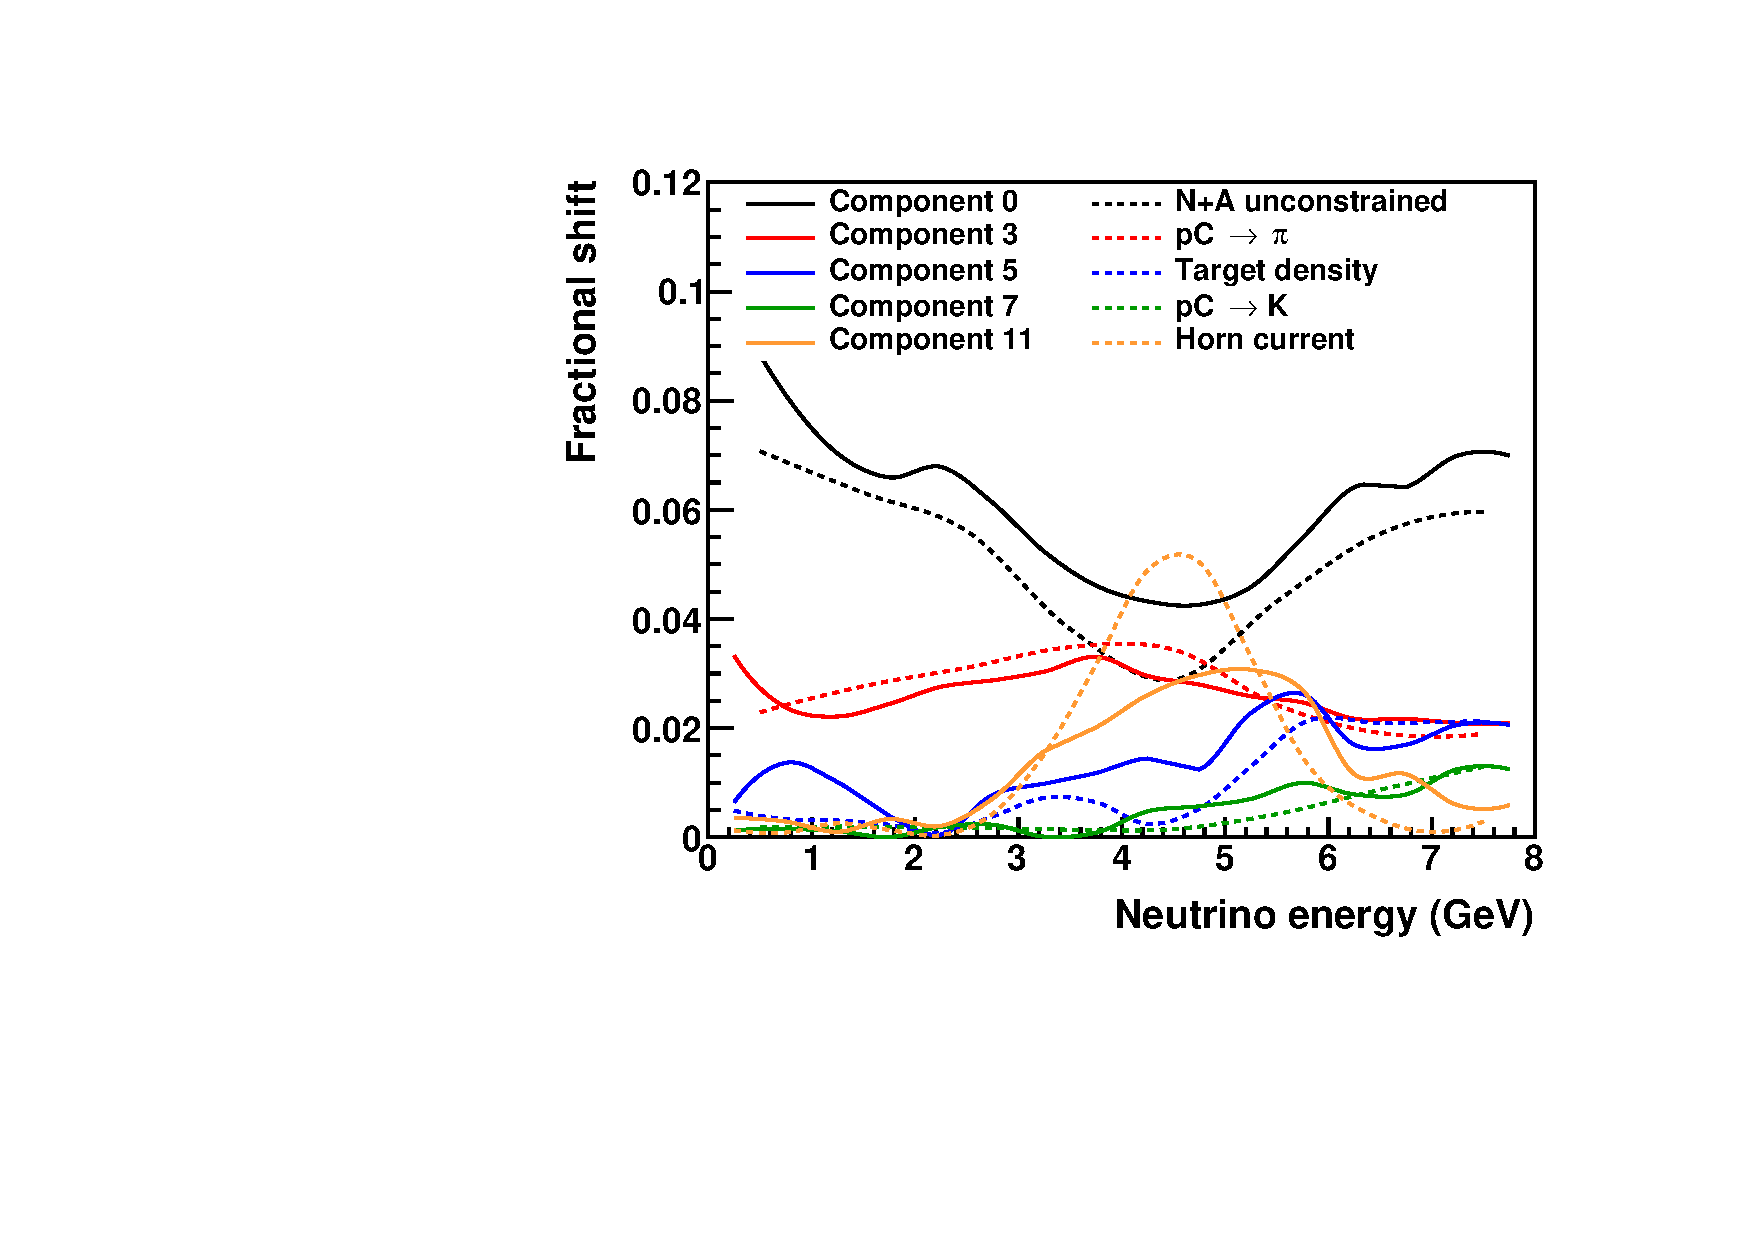
\includegraphics[width=0.9\textwidth]{Flux_Unc_PCA.pdf}
\end{dunefigure}

%\subsection{Assumed measurements and constraints}
%\label{sec:assumedconstraints}

%The oscillation analysis presented here is intended to demonstrate the full potential of \dword{dune}, including constraints from the full suite of near detectors described in the Executive Summary. In addition to the \numu and \anumu \dword{cc} spectra explicitly used in these fits, the \dword{lar} \dword{tpc} is also expected to measure many different exclusive final-state \dword{cc} samples, including 1$\pi^{\pm}$, 1$\pi^{0}$, and multi-pion production. Measurements can be made as a function of many kinematic quantities in addition to $E_{\nu}$ and $y$, for example four-momentum transfer to the nucleus, $Q^{2}$, lepton angle, or final-state pion kinematics. The \dword{lar} \dword{tpc} is also expected to measure the sum of \nue and \anue \dword{cc} scattering, as well as \dword{nc} events. Direct flux measurements will also be possible with neutrino-electron scattering and the low-$\nu$ technique.

%In addition to the many on-axis \dword{lar} samples, a complementary set of neutrino-Argon measurements is expected from the \dword{hpg} \dword{tpc}. This detector will be sensitive to charged tracks at kinetic energies of just a few MeV, enabling the study of nuclear effects in unprecedented detail. It will also sign-select all charged particles, with nearly perfect pion-proton separation from dE/dx out to over 1 GeV/c momentum, so that high-purity measurements of CC1$\pi^{+}$ and CC1$\pi^{-}$ are possible. It may be possible to directly measure neutron energy spectra from time of flight using the \dword{hpg} \dword{tpc} coupled to a high-performance \dword{ecal}. The 3DST-S will measure neutrino-carbon scattering and neutron production while ensuring excellent beam stability.

%The \dword{lar} and \dword{mptdet} will also move off-axis to measure neutrino-Argon interactions in many different fluxes. This will provide a direct constraint on the relationship between neutrino energy and visible energy in \dword{lar}. By taking linear combinations of spectra at many off-axis positions out to 33 m, it is possible to reproduce the expected \dword{fd} energy spectrum for a given set of oscillation parameters and directly measure visible energy.

%All of these measurements are critical to the \dword{dune} program. However, due to the timing of the \dword{nd} design process, there is not sufficient time to explicitly include all of these samples and show their impact on oscillation sensitivity. Instead, we assume a model for cross sections and detector effects that implicitly includes these constraints, and leave the justification for this assumption to the \dword{nd} \dword{tdr}.

%The most critical assumption is our use of the \dword{genie} event generator as a model for neutrino-Argon interactions. While our uncertainty model described in Section~\ref{sec:nu-osc-05} significantly expands on \dword{genie} uncertainties, it is still not possible to include every possible potential discrepancy between our model and Nature. To determine the sensitivity with the far detector alone, it is not sufficient to simply remove the near detector constraint from our fits, as the analysis implicitly relies on the broader near detector program to ensure that the model is correct up to the parameter uncertainties we include. This assumption is evidently invalid in the case where there is not a high-performance near detector.

%little editing can make it better, for example: 
%The uncertainty model described in Section~\ref{sec:nu-osc-05} significantly expands with respect to the default \dword{genie} uncertainties, however it is not possible to include every possible potential discrepancy between the model and the true parameters of nature. To determine the sensitivity with the far detector alone, it is not sufficient to remove the near detector constraint, as the analysis implicitly relies on the broader near detector program to ensure that the model is correct up to the parameter uncertainties we include. In fact any self-consistent analysis that one can propose at this stage requires a high-performance near detector.

%To estimate the sensitivity in \dword{fd}-only case, we construct a plausible alternative sample based on the \dword{nuwro} event generator. Fitting only the \dword{fd} samples gives a good quality of fit, but at the wrong best-fit oscillation parameters. This would result in a bias, but one which is easy to observe at the \dword{nd}. The bias is added as an additional uncertainty as an example of an effect which is not covered by our model. This is described in Section~\ref{sec:ndbias}.